\documentclass[11pt,a4paper]{article}

% ── Packages ──────────────────────────────────────────────────────
\usepackage[a4paper, margin=2.5cm]{geometry}
\usepackage{graphicx}
\usepackage{booktabs}
\usepackage{array}
\usepackage{tabularx}
\usepackage{longtable}
\usepackage{xcolor}
\usepackage{colortbl}
\usepackage{fancyhdr}
\usepackage{titlesec}
\usepackage{enumitem}
\usepackage{natbib}
\usepackage{hyperref}
\usepackage{setspace}
\usepackage{parskip}
\usepackage{multirow}
\usepackage{makecell}
\usepackage{tikz}
\usepackage{mdframed}
\usepackage{caption}
\usepackage{float}

% ── FIX: spacing between header and content ───────────────────────
\setlength{\headsep}{50pt}

% ── Colours ───────────────────────────────────────────────────────
\definecolor{bcublue}{RGB}{31,56,100}
\definecolor{midblue}{RGB}{46,117,182}
\definecolor{lightblue}{RGB}{214,228,240}
\definecolor{tablegrey}{RGB}{242,242,242}
\definecolor{darkgrey}{RGB}{89,89,89}

% ── Font ──────────────────────────────────────────────────────────
\usepackage{helvet}
\renewcommand{\familydefault}{\sfdefault}

% ── Section formatting ────────────────────────────────────────────
\titleformat{\section}
  {\color{bcublue}\large\bfseries}{{\thesection}}{1em}{}
  [\vspace{2pt}\color{midblue}\titlerule]

\titleformat{\subsection}
  {\color{midblue}\normalsize\bfseries}{\thesubsection}{1em}{}

\titleformat{\subsubsection}
  {\color{darkgrey}\normalsize\bfseries}{\thesubsubsection}{1em}{}

% ── Header / Footer ───────────────────────────────────────────────
\pagestyle{fancy}
\fancyhf{}
\renewcommand{\headrulewidth}{0.4pt}
\renewcommand{\headrule}{\hbox to\headwidth{%
  \color{midblue}\leaders\hrule height \headrulewidth\hfill}}
\fancyhead[L]{\small\color{darkgrey} CMP6230 Coursework 1}
\fancyhead[R]{\includegraphics[height=35pt]{logo.png}}
\fancyfoot[C]{\small\color{darkgrey}\thepage}

% ── Hyperlinks ────────────────────────────────────────────────────
\hypersetup{
  colorlinks=true,
  linkcolor=midblue,
  urlcolor=midblue,
  citecolor=midblue
}

% ── natbib: author-year citations ─────────────────────────────────
\setcitestyle{authoryear, open={(}, close={)}}

% ── Table helpers ─────────────────────────────────────────────────
\newcolumntype{L}[1]{>{\raggedright\arraybackslash}p{#1}}
\newcolumntype{C}[1]{>{\centering\arraybackslash}p{#1}}

% ── ML target box ─────────────────────────────────────────────────
\newmdenv[
  backgroundcolor=lightblue,
  linecolor=midblue,
  linewidth=1pt,
  leftmargin=0pt,
  rightmargin=0pt,
  innerleftmargin=8pt,
  innerrightmargin=8pt,
  innertopmargin=6pt,
  innerbottommargin=6pt,
]{mlbox}

% ══════════════════════════════════════════════════════════════════
\begin{document}

% ── COVER PAGE ────────────────────────────────────────────────────
\thispagestyle{empty}

\begin{center}
  \includegraphics[width=200pt]{logo.png}\\[0.4cm]

  \textbf{\Large\color{black} BIRMINGHAM CITY UNIVERSITY}\\[0.3cm]
  {\color{darkgrey} Faculty of Computing, Engineering and the Built Environment}\\[1.5cm]

  {\large\bfseries\color{black} CMP6230: Data Management and ML Operations}\\[0.3cm]
  {\color{darkgrey} Coursework Task 1}\\[2cm]

  {\Huge\bfseries\color{black} Data Analytics Pipeline\\[0.3cm] Planning and Design}\\[3cm]

  \begin{tabular}{rl}
    \textbf{Student Name:}    & Shekhar Lamichhane Magar \\[4pt]
    \textbf{Student ID:}      & 23189647 \\[4pt]
    \textbf{Course:}          & BSc (Hons) Computer and Data Science \\[4pt]
    \textbf{Submission Date:} & 17th May 2026 \\[4pt]
    \textbf{Email:}           & shekhar\_23189647@sunway.edu.np \\[4pt]
    \textbf{Word Count:}      & $\approx$1000 \\
  \end{tabular}
\end{center}

\newpage

% ── TABLE OF CONTENTS ─────────────────────────────────────────────
\tableofcontents
\newpage


\listoffigures
\listoftables
\newpage

% ══════════════════════════════════════════════════════════════════
\section{Introduction}

For this coursework, I evaluated three datasets and designed a data analytics pipeline 
around the most practical one. I chose the E-Commerce Behavior Dataset (8,000 users) because 
it has a straightforward classification target—predicting whether a customer clicks an ad. 
No feature engineering needed, no missing labels. Just clean data ready to work with.

The pipeline I designed covers the full lifecycle: data ingestion, preprocessing, model 
training, deployment to production, and monitoring for performance drift. It's meant to 
support both data scientists exploring the data and automated retraining when performance 
starts to degrade.

% ══════════════════════════════════════════════════════════════════
\section{Candidate Datasets Analysis}

% ── 2.1 ──────────────────────────────────────────────────────────
\subsection{Dataset 1: AI Impact on Job Market 2024--2030}

This dataset from Kaggle user sahilislam007 \citep{sahilislam2024} tracks how AI will 
affect different job roles over the next few years. It pulls together labour market 
projections from World Economic Forum reports. The file is a single CSV with 10 columns 
and around 500 rows. You get job titles, industries, salary ranges, education requirements, 
and AI exposure levels. 

The main appeal? Lots of categorical features to work with. But the target variable—AI Impact 
Level (High/Medium/Low)—is somewhat subjective. It's not like a clear binary outcome. Plus, 
500 rows felt small for splitting into train and test sets. I considered using it, but the 
ordinal nature of the target made me hesitant.

\vspace{0.3cm}
\begin{table}[H]
\centering
\caption{Dataset 1 Column Analysis}
\small
\begin{tabular}{L{3.5cm} L{5cm} L{2cm} L{2cm}}
\toprule
\rowcolor{black}
\textcolor{white}{\textbf{Column Name}} &
\textcolor{white}{\textbf{Description}} &
\textcolor{white}{\textbf{Measurement}} &
\textcolor{white}{\textbf{Data Type}} \\
\midrule
Job Title              & Job role name                  & Nominal & Categorical \\
\rowcolor{tablegrey}
Industry               & Sector of employment           & Nominal & Categorical \\
Job Status             & Employment type                & Nominal & Categorical \\
\rowcolor{tablegrey}
AI Impact Level        & AI exposure (High/Med/Low)     & Ordinal & Categorical \\
Median Salary (USD)    & Annual salary estimate         & Ratio   & Float \\
\rowcolor{tablegrey}
Required Education     & Minimum qualification          & Ordinal & Categorical \\
Experience Required    & Min.\ years of experience      & Ratio   & Integer \\
\rowcolor{tablegrey}
Job Openings (2024)    & Current openings               & Ratio   & Integer \\
Projected Openings (2030) & Forecasted openings         & Ratio   & Integer \\
\rowcolor{tablegrey}
Remote Work?           & Remote eligibility             & Nominal & Boolean \\
\bottomrule
\end{tabular}
\end{table}

\begin{mlbox}
\textbf{\color{black} ML Targets}\\
\textbf{Target:} AI Impact Level (multi-class: High / Medium / Low).\\
\textbf{Predictors:} Industry, Salary, Education, Experience, Remote Work.
\end{mlbox}

\vspace{0.5cm}

% ── 2.2 ──────────────────────────────────────────────────────────
\subsection{Dataset 2: E-Commerce Behavior Dataset (8,000 Users)
            \textnormal{\textit{[PRIMARY]}}}

I found this one on Kaggle (user asifxzaman) and it immediately stood out. It contains 
session data from 8,000 e-commerce users with their browsing habits, purchase history, 
and—most importantly—whether they clicked an ad or not. The dataset is around 300 kB, 
clean CSV format, 8,000 rows by 10 columns. Perfect size for training without needing 
distributed computing.

Each row represents one user session. You get their age, gender, device type, how long 
they spent on the site, pages visited, past purchases, items in cart, whether they saw 
a discount, and finally: did they click the ad? That last column is exactly what I need 
to predict. Binary outcome, no ambiguity.

\vspace{0.3cm}
\begin{table}[H]
\centering
\caption{Dataset 2 Column Analysis}
\small
\begin{tabular}{L{3.5cm} L{5cm} L{2cm} L{2cm}}
\toprule
\rowcolor{black}
\textcolor{white}{\textbf{Column Name}} &
\textcolor{white}{\textbf{Description}} &
\textcolor{white}{\textbf{Measurement}} &
\textcolor{white}{\textbf{Data Type}} \\
\midrule
user\_id             & Unique session identifier      & Nominal & Integer \\
\rowcolor{tablegrey}
age                  & User age in years              & Ratio   & Integer \\
gender               & Self-reported gender           & Nominal & Categorical \\
\rowcolor{tablegrey}
device\_type         & Access device type             & Nominal & Categorical \\
time\_on\_site       & Minutes on platform            & Ratio   & Float \\
\rowcolor{tablegrey}
pages\_viewed        & Number of pages visited        & Ratio   & Integer \\
previous\_purchases  & Total past purchases           & Ratio   & Integer \\
\rowcolor{tablegrey}
cart\_items          & Items currently in cart        & Ratio   & Integer \\
discount\_seen       & Discount presented (0/1)       & Nominal & Boolean \\
\rowcolor{tablegrey}
\textbf{ad\_clicked} & \textbf{Ad clicked --- TARGET (0/1)} & Nominal & Boolean \\
\bottomrule
\end{tabular}
\end{table}

% ── ERD Diagram ───────────────────────────────────────────────────
\begin{figure}[H]
\centering
\begin{tikzpicture}[scale=0.9]
  % Header
  \draw[fill=midblue, draw=midblue, line width=2pt]
    (0,0) rectangle (11,0.85);
  \node[text=white, font=\bfseries\Large] at (5.5,0.425) {USER\_SESSION};

  % Rows
  \foreach \i/\attr/\fill in {
    1/{user\_id \quad INT \quad PRIMARY KEY}/white,
    2/{age \quad INT}/white,
    3/{gender \quad VARCHAR}/white,
    4/{device\_type \quad VARCHAR}/white,
    5/{time\_on\_site \quad FLOAT}/white,
    6/{pages\_viewed \quad INT}/white,
    7/{previous\_purchases \quad INT}/white,
    8/{cart\_items \quad INT}/white,
    9/{discount\_seen \quad BOOLEAN}/white,
    10/{ad\_clicked \quad BOOLEAN \quad \textrightarrow\ TARGET}/lightblue
  }{
    \pgfmathsetmacro\ypos{-0.85 - (\i-1)*0.58}
    \fill[\fill] (0,\ypos) rectangle (11,{\ypos-0.55});
    \draw[midblue, line width=0.6pt] (0,\ypos)
      rectangle (11,{\ypos-0.55});
    \node[font=\ttfamily\small, anchor=west]
      at (0.3,{\ypos-0.275}) {\attr};
  }
\end{tikzpicture}
\caption{Entity-Relationship Diagram (ERD) ---
         E-Commerce Behavior Dataset Schema}
\label{fig:erd}
\end{figure}

\begin{mlbox}
\textbf{\color{black} ML Targets}\\
\textbf{Target:} ad\_clicked (binary: 0 = No, 1 = Yes).\\
\textbf{Predictors:} age, gender, device\_type, time\_on\_site, pages\_viewed,
previous\_purchases, cart\_items, discount\_seen.
\end{mlbox}

\vspace{0.5cm}

% ── 2.3 ──────────────────────────────────────────────────────────
\subsection{Dataset 3: US Tariff and Trade War Impact Dataset (2018--Present)}

The third option is a time-series dataset tracking how US-China trade tariffs have affected 
financial markets. Daily records from 2018 to now, pulling in S\&P 500 closing prices, 
currency rates, crude oil futures, steel prices, all that economic stuff. It's aggregated 
from Yahoo Finance and FRED, hosted on Kaggle by user belbino.

At first I thought this could work well—lots of continuous variables, real-world data, 
interesting story behind it. But then I realized the problem: there's no built-in target 
variable. I'd have to engineer one (like ``S\&P 500 goes up tomorrow?''), and that adds 
another layer of complexity. Plus time-series data requires walk-forward validation to avoid 
data leakage. For a first coursework, that seemed like overkill compared to the other options.

\vspace{0.3cm}
\begin{table}[H]
\centering
\caption{Dataset 3 Column Analysis}
\small
\begin{tabular}{L{3.5cm} L{5cm} L{2cm} L{2cm}}
\toprule
\rowcolor{black}
\textcolor{white}{\textbf{Column Name}} &
\textcolor{white}{\textbf{Description}} &
\textcolor{white}{\textbf{Measurement}} &
\textcolor{white}{\textbf{Data Type}} \\
\midrule
date                 & Trading date                   & Nominal & Date  \\
\rowcolor{tablegrey}
sp500                & S\&P 500 closing price         & Ratio   & Float \\
shanghai\_composite  & Shanghai Composite index       & Ratio   & Float \\
\rowcolor{tablegrey}
dxy                  & US Dollar Index                & Ratio   & Float \\
usd\_cny             & USD to Chinese Yuan rate       & Ratio   & Float \\
\rowcolor{tablegrey}
crude\_oil\_wti      & WTI crude oil futures          & Ratio   & Float \\
steel\_future        & Steel futures price            & Ratio   & Float \\
\rowcolor{tablegrey}
aluminum\_future     & Aluminium futures price        & Ratio   & Float \\
soybeans             & Soybean futures price          & Ratio   & Float \\
\bottomrule
\end{tabular}
\end{table}

\begin{mlbox}
\textbf{\color{black} ML Targets}\\
\textbf{Target:} Would need to engineer: sp500\_direction (up/down next day).\\
\textbf{Limitation:} No pre-built target; time-series validation is tricky.
\end{mlbox}

\newpage

% ══════════════════════════════════════════════════════════════════
\section{Dataset Selection Justification}

\textbf{Selected Dataset: E-Commerce Behavior Dataset (Dataset 2).}

\begin{table}[H]
\centering
\caption{Candidate Dataset Comparison}
\small
\begin{tabular}{L{4cm} L{2cm} L{4cm} L{2.5cm}}
\toprule
\rowcolor{bcublue}
\textcolor{white}{\textbf{Dataset}} &
\textcolor{white}{\textbf{Records}} &
\textcolor{white}{\textbf{ML Task}} &
\textcolor{white}{\textbf{Decision}} \\
\midrule
AI Impact on Job Market
  & $\sim$500
  & Multi-class (ordinal target, subjective)
  & Rejected \\
\rowcolor{lightblue}
\textbf{\color{bcublue}E-Commerce Behavior}
  & \textbf{8,000}
  & \textbf{Binary classification (pre-labelled)}
  & \textbf{\color{bcublue}Selected} \\
US Tariff Trade War
  & 2,500+ daily
  & Time-series (no pre-defined target)
  & Rejected \\
\bottomrule
\end{tabular}
\end{table}

Here's why the e-commerce dataset made sense:

\begin{itemize}[leftmargin=1.5em, itemsep=3pt]
  \item \textbf{Ready-made target:} The \texttt{ad\_clicked} column is 0 or 1. No engineering, no ambiguity. Unlike the tariff dataset, I don't need to invent a target.
  \item \textbf{8,000 rows is solid:} Big enough to do meaningful train/test splits (80/20) without touching distributed systems. Dataset 1 had only 500 rows.
  \item \textbf{Mixed feature types:} Demographics, behavior, transactional data—gives me lots to work with in feature engineering.
  \item \textbf{Real business value:} Click-through prediction is a genuinely important problem in digital marketing. Not just an academic exercise.
  \item \textbf{Standard classification:} No special validation tricks needed. Regular cross-validation works.
\end{itemize}

% ══════════════════════════════════════════════════════════════════
\section{Data Analytics Pipeline Design}

\subsection{Pipeline Overview}

\begin{figure}[H]
    \centering
    \includegraphics[width=\textwidth, height=0.45\textheight, keepaspectratio]{pipeline.png}
    \caption{End-to-End MLOps Pipeline Architecture
             (Orchestrated by Apache Airflow)}
    \label{fig:mlops_pipeline}
\end{figure}

I built this pipeline using Apache Airflow to orchestrate all the moving parts. Here's the 
tech stack: Python handles most of the processing, MLflow tracks experiments and model versions, 
and Evidently AI watches for data drift. Each stage feeds into the next automatically.

\subsection{Getting Data In (Ingestion)}

The ingestion stage is where everything starts. I pull the CSV from Kaggle automatically using 
their API—no manual downloads. When Airflow kicks off a run, it grabs the latest file and 
runs validation on it right away. I use Great Expectations for schema checks: \texttt{user\_id} 
has to be unique, \texttt{ad\_clicked} must be 0 or 1, age between 13--100. Pretty strict, 
but that's the point. Bad data early on ruins everything downstream, so I'd rather fail fast.

If validation passes, rows get bulk-loaded into a MariaDB staging table with metadata: 
\texttt{ingestion\_ts} (when it arrived) and \texttt{pipeline\_run\_id} (which batch it was). 
This matters more than it sounds. Six months from now, if something's broken, I can go back 
and say "that batch was the problem." Full traceability.

\subsection{Cleaning and Preparing Data}

Once valid data is in the system, the real work starts. Missing values? Fill them with column 
medians—quick and usually works. Categorical variables (\texttt{gender}, \texttt{device\_type}) 
get one-hot encoded. Numeric columns get StandardScaler applied—nothing fancy, just puts 
everything on the same scale so the model doesn't get confused by age ranging 13--100 while 
time on site is 5--600.

I also cooked up a feature: \texttt{engagement\_score = (pages\_viewed × time\_on\_site) / 
(cart\_items + 1)}. It's basically "how many pages per minute did they look at relative to 
their cart." Could be garbage, could be gold—I'll find out during model training. Final output 
is a feature table split 80/20 into train and test (stratified, so I don't accidentally get all 
clickers in train and all non-clickers in test).

\subsection{Training Models}

For model development, I use Jupyter notebooks in an Anaconda environment. I try three algorithms: 
Logistic Regression (simple baseline), Random Forest (captures non-linearity), and XGBoost 
(usually performs best). MLflow tracks every run—parameters, metrics like accuracy and F1, 
and the trained model artifacts. Hyperparameters get tuned with Optuna. The best model 
automatically gets registered in MLflow's model registry.

\subsection{Putting Models in Production}

Once I've found something that works, it's time to actually use it. I build a REST API around 
the model using FastAPI—takes user session data in JSON format, spits out a prediction and 
confidence score. Wrap it in Docker for consistency across environments. This endpoint can scale 
and handle real traffic. If Airflow detects drift and triggers a retrain, it automatically 
deploys the new model without any manual intervention. One less thing to worry about at 3am.

\subsection{Watching for Problems (Monitoring)}

This is honestly the most important part, though nobody gets excited about it. I use Evidently AI 
to monitor data drift. Every week I calculate Population Stability Index (PSI) on every feature 
and track ROC-AUC on new predictions. The reason? E-commerce audiences change. New student batches 
arrive each semester, spending patterns shift with seasons, device preferences drift as phones 
get updated. The model trained on last year's users will quietly perform worse on this year's users 
without any obvious errors. You only notice when revenue drops. So if PSI climbs above 0.2 or 
ROC-AUC falls more than 0.05, Airflow automatically alerts me and queues up a retrain. Better 
to catch it early.

\newpage

% ══════════════════════════════════════════════════════════════════
\section{Data Storage Plan}

The input dataset is the E-Commerce Behavior Dataset: 10 columns, 8,000 rows, CSV format. 
Single flat table—see the ERD in Figure~\ref{fig:erd} and Table~2.

For storage, I'm using a One Big Table (OBT) schema in MariaDB ColumnStore. ColumnStore is 
column-oriented, which is optimal for ML feature scans. I initially planned a simple SQLite 
setup, but then realized that columnar engines are much faster for the kinds of queries I'd 
be running—scanning many rows and aggregating columns to extract features.

I considered a Star Schema (fact + dimension tables), but that would require joins. In a 
columnar engine, joins re-materialize data row-by-row, which defeats the purpose of having 
columns. With a single entity (just user sessions), OBT is cleaner and faster.

\begin{figure}[H]
\centering
\begin{tikzpicture}
  \draw[fill=black, draw=midblue, line width=1pt]
    (0,0) rectangle (12,0.7);
  \node[text=white, font=\bfseries] at (6,0.35)
    {user\_session\_obt \quad
     (MariaDB ColumnStore --- OLAP, port 3308)};

  \foreach \i/\attr/\tag/\fill in {
    1/{user\_id \quad INT \quad PRIMARY KEY}/{}/white,
    2/{age \quad INT}/{[PREDICTOR]}/tablegrey,
    3/{gender \quad VARCHAR(20)}/{[PREDICTOR]}/white,
    4/{device\_type \quad VARCHAR(30)}/{[PREDICTOR]}/tablegrey,
    5/{time\_on\_site \quad FLOAT}/{[PREDICTOR]}/white,
    6/{pages\_viewed \quad INT}/{[PREDICTOR]}/tablegrey,
    7/{previous\_purchases \quad INT}/{[PREDICTOR]}/white,
    8/{cart\_items \quad INT}/{[PREDICTOR]}/tablegrey,
    9/{discount\_seen \quad TINYINT(1)}/{[PREDICTOR]}/white,
    10/{ad\_clicked \quad TINYINT(1)}/{[TARGET]}/lightblue,
    11/{ingestion\_ts \quad DATETIME}/{[METADATA]}/tablegrey,
    12/{pipeline\_run\_id \quad VARCHAR(50)}/{[METADATA]}/white
  }{
    \fill[\fill] (0,{-(\i-1)*0.45})
      rectangle (12,{-(\i-1)*0.45-0.42});
    \draw[midblue, line width=0.5pt] (0,{-(\i-1)*0.45})
      rectangle (12,{-(\i-1)*0.45-0.42});
    \node[font=\ttfamily\small, anchor=west]
      at (0.2,{-(\i-1)*0.45-0.21}) {\attr};
    \node[font=\ttfamily\small\color{darkgrey}, anchor=east]
      at (11.8,{-(\i-1)*0.45-0.21}) {\tag};
  }
\end{tikzpicture}
\caption{OBT Schema --- MariaDB ColumnStore Analytical Store
         (\texttt{user\_session\_obt})}
\label{fig:obt}
\end{figure}

\begin{table}[H]
\centering
\caption{Storage Structure Comparison}
\small
\begin{tabular}{L{3cm} L{5.5cm} L{4cm}}
\toprule
\rowcolor{bcublue}
\textcolor{white}{\textbf{Structure}} &
\textcolor{white}{\textbf{Benefits}} &
\textcolor{white}{\textbf{Drawbacks}} \\
\midrule
\textbf{\color{bcublue}OBT (CHOSEN)}
  & No joins; optimal for columnar ML feature scans; fastest for
    MariaDB ColumnStore analytics
  & No referential integrity; harder to extend with new entities \\
\rowcolor{tablegrey}
Star Schema
  & Separates concerns; analyst-friendly
  & Requires joins across dimension/fact tables; joins
    re-materialise rows in ColumnStore, negating columnar advantage \\
Snowflake Schema
  & More normalised; less redundancy
  & Complex joins; harder to query \\
\rowcolor{tablegrey}
Normalised (3NF)
  & Full integrity; no redundancy
  & Many joins for every ML query; slowest for ColumnStore
    access patterns \\
\bottomrule
\end{tabular}
\end{table}

On the infrastructure side, I'm running two Docker containers on Ubuntu. One is regular 
MariaDB (port 3306)—that's for transactional writes during ingestion. The other is MariaDB 
ColumnStore (port 3308)—that's the analytical store where I actually do my ML work. An Airflow 
DAG transfers clean rows from OLTP to OLAP on a schedule. In production, I'd migrate this to 
Google BigQuery or Snowflake.

\subsection{ETL Process}

Starting with the Extract phase: I pull CSV from Kaggle via their API. Great Expectations 
validates three rules: \texttt{user\_id} must be unique (no duplicate sessions), \texttt{ad\_clicked} 
can only be 0 or 1, age needs to fall in the 13--100 range. If anything fails, the pipeline 
stops and I get an alert.

Transform is the real work. Missing values get filled with column medians (not ideal, but 
fast). I one-hot encode \texttt{gender} and \texttt{device\_type} for the model. Numeric 
columns get scaled with StandardScaler. Then I create the engagement feature and some age 
bands (though I'm still not sure those age bands help—might clean them up later). Finally, 
stratified 80/20 split on train/test so I don't accidentally bias my results.

For Load: I bulk-insert validated rows into MariaDB OLTP (\texttt{raw\_user\_sessions}), then 
Airflow transfers clean data to ColumnStore (\texttt{user\_session\_obt}) on a schedule. I log 
everything—timestamp, row counts, validation status—to \texttt{pipeline\_log} for auditing. That 
way if something breaks six months from now, I have the trail.

% ══════════════════════════════════════════════════════════════════
\section{Iterative Refinement \& Reflection}

\subsubsection*{How I Got Here}

\textbf{First attempt:} I started with a simple flat OBT design and a basic pandas-only pipeline 
using SQLite. Honestly, I didn't think much beyond "get the data, clean it, train a model."

\textbf{Second pass:} Once I started thinking about actually running this at scale, I realized 
SQLite would bottleneck. Switched to MariaDB ColumnStore after reading about how columnar 
engines optimize for ML workloads. I initially sketched out a Star Schema, but then worked 
through a couple of queries—realized joins would destroy the columnar advantage for my dataset. 
Scrapped it and stuck with OBT \citep{zaitsev2021}.

\textbf{Third version:} Added proper experiment tracking with MLflow and drift detection with 
Evidently AI. Without monitoring, you don't know when things break.

\subsubsection*{What I Learned}

The biggest lesson: storage engine choice has to come first. The schema that's optimal for 
MariaDB ColumnStore (OBT with no joins) is completely different from what's optimal for a 
row-based RDBMS. If I'd designed the schema first without thinking about the engine, I'd have 
built something that doesn't work well with ColumnStore.

Also—designing for multiple consumers (both ad-hoc scientist queries and automated training) 
forced better structural decisions. Single-consumer designs often have blind spots.

On the monitoring side: I initially thought I'd just watch the model's output metrics. Wrong. 
The real killer is feature drift. In e-commerce, user demographics shift seasonally—new cohorts 
arrive, old patterns fade. A model trained on last year's student users performs terribly on 
this year's users. You have to check feature distributions, not just model metrics.

\subsubsection*{What's Next?}

If I had more runway on this project, I'd do a few things. Right now the data is pretty bare-bones—just user 
demographics and behavior. Adding product category or time-of-day would probably help the model distinguish 
patterns better. The batch ingestion works fine now, but Kafka streaming would be nicer if this was a live 
system with real e-commerce traffic. I should also set up proper data lineage tracking with something like 
Apache Atlas—for compliance and just knowing where things came from. And MLflow's backend is currently SQLite, 
which is fine for development but would choke with multiple users. Moving it to MariaDB would be a quick win 
for production.

\newpage

% ══════════════════════════════════════════════════════════════════
% REFERENCES — automatically generated from references.bib
% ══════════════════════════════════════════════════════════════════
\addcontentsline{toc}{section}{References}
\bibliographystyle{plainnat}
\bibliography{references}

\end{document}
